\chapter{MOEA Random Seed Analysis}
\label{appendix-seedanalysis}

This appendix considers the impact of the random seed to the results of the MOEA-based search process for each method. The random seed influences the initial population selection for each repetition, which uses Latin Hypercube Sampling, among other functionality. Analysis is broken down per robust decision support method. 

\section{MORDM} \label{seedanalysis-mordm}
The results of the random seed analysis for each MORDM-based analysis is shown in \cref{fig:pareto-mordm} and includes three types of plots. The first column displays the size of the identified non-dominated Pareto front size for each search repetition. The second column shows hypervolume of the final non- dominated policy set. The final column compares the size of the non-dominated set of policy alternatives to the hypervolume of each set. 

\begin{figure}[H]
    \centering
    
    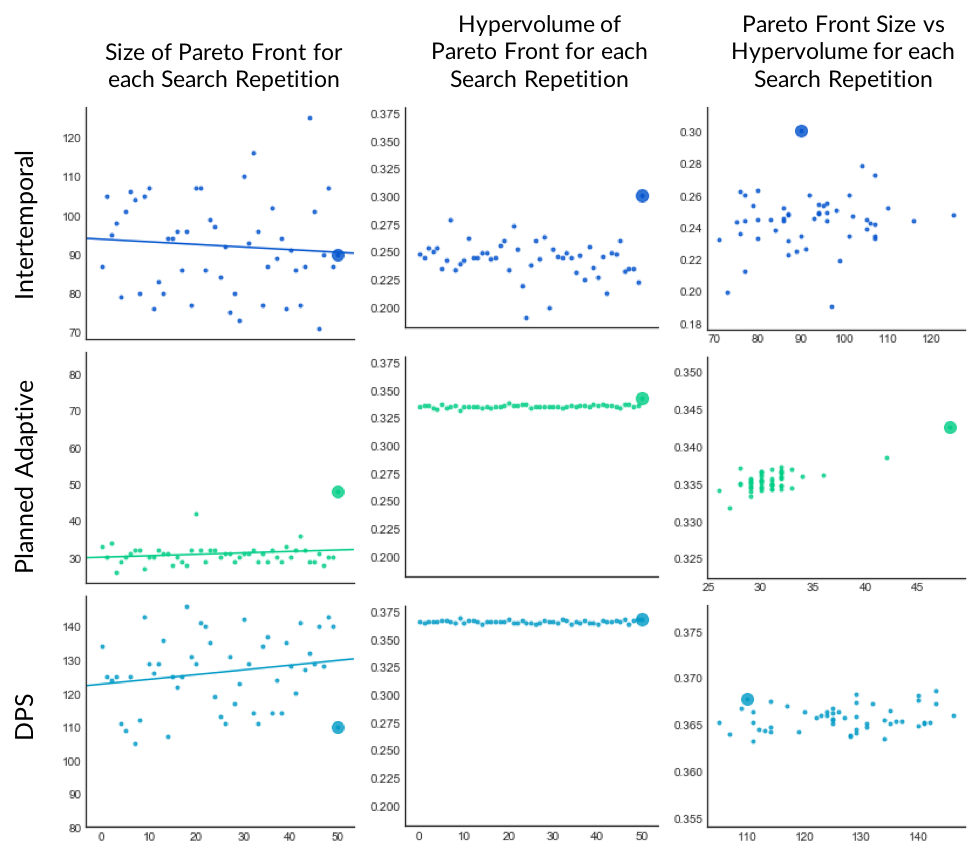
\includegraphics[width=0.75\textwidth]{appendices/seed_analysis/paretosize_mordm}
    \caption[Random seed analysis for all uses of MORDM]{Random seed analysis for the MORDM robust decision support method. The large circle represents the set of non-dominated alternatives that combines the results from each search repetition.}
    \label{fig:pareto-mordm}
\end{figure}

The final combined non-dominated set of policy alternatives for the intertemporal analysis yields a number of policy alternatives that is similar to the results found in each search repetition. However, as indicated by the plot in the second column, that final combined set does result in a larger hypervolume than a single search repetition. This indicates that using multiple search repetitions did improve the diversity of the final policy set without increasing the size of the set, providing a stronger foundation for the future steps in the analysis. 

In contrast, despite the combined non-dominated set of alternatives containing a larger number of policies, the hypervolume was not increased with respect to the planned adaptive DPS model variation. In fact, the hypervolume of each search repetition is extremely constant, indicating that the random seed does not have any real impact on the diversity of the final non-dominated set of policy alternatives. 

Finally, the combined results for the DPS model variation include a smaller number of policy alternatives than most of the stand-alone search repetitions. At the same time, that front is able to maintain a similar hypervolume as each stand-alone repetition. This indicates that considering multiple repetitions of an MOEA-based search leads to a smaller set of non-dominated alternatives that are just as diverse as an individual repetition. Such a smaller set may prove easier for decision makers to manage in the later steps of an analysis. 

\section{Multi-Scenario MORDM}

\begin{figure}[H]
    \centering
    
    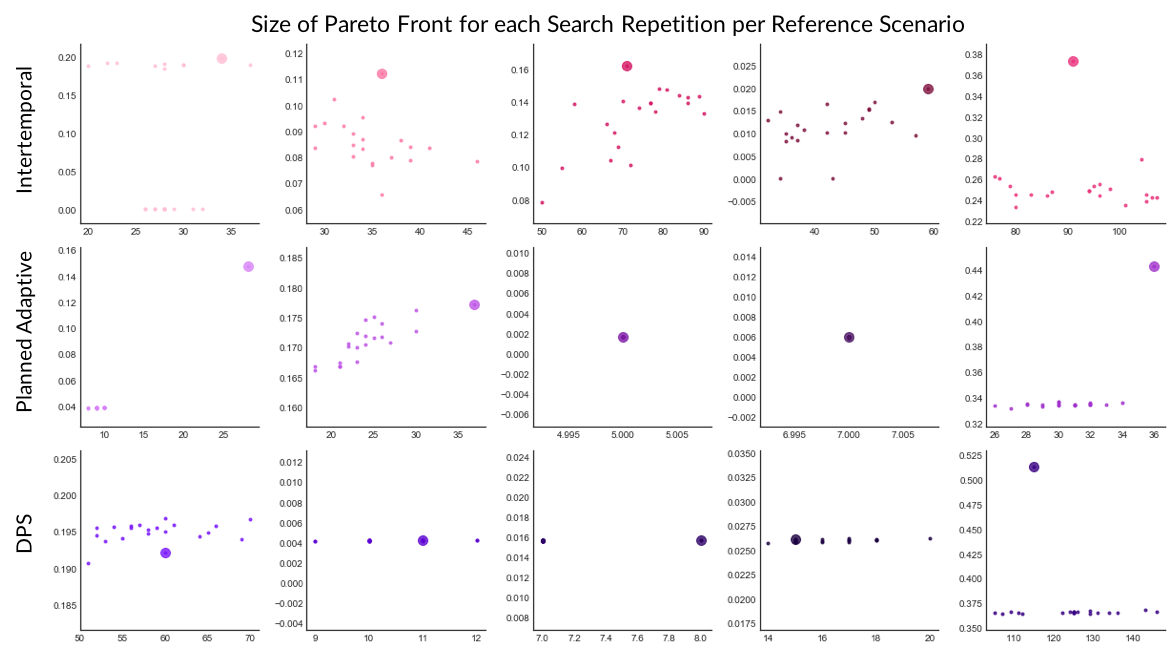
\includegraphics[width=0.95\textwidth]{appendices/seed_analysis/paretosize_multi_front}
    \caption[Pareto front size across search repetitions for multi-scenario MORDM]{Size of the pareto front for each search repetition of all multi-scenario MORDM analyses.}
    \label{fig:pareto-multi-size}
\end{figure}

\begin{figure}[H]
    \centering
    
    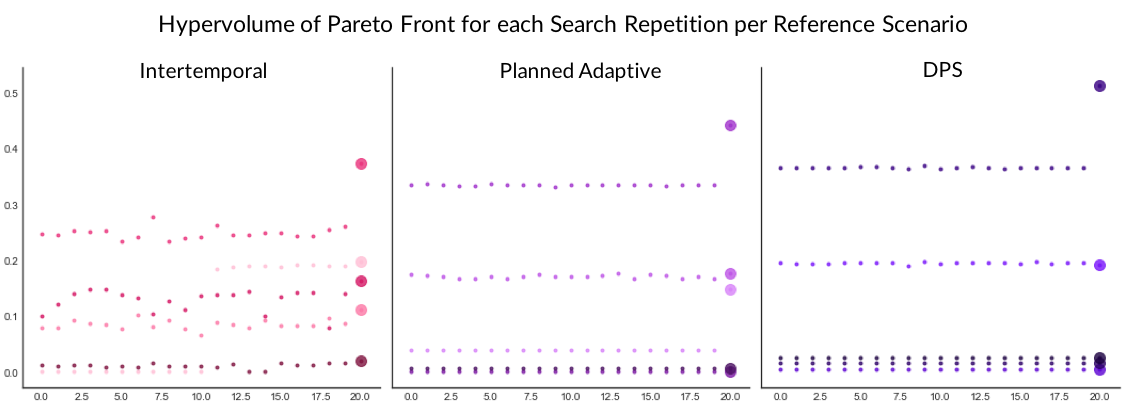
\includegraphics[width=0.95\textwidth]{appendices/seed_analysis/paretosize_multi_hypervolume}
    \caption{Hypervolume of the pareto front for all multi-scenario MORDM analyses.}
    \label{fig:pareto-multi-volume}
\end{figure}

\begin{figure}[H]
    \centering
    
    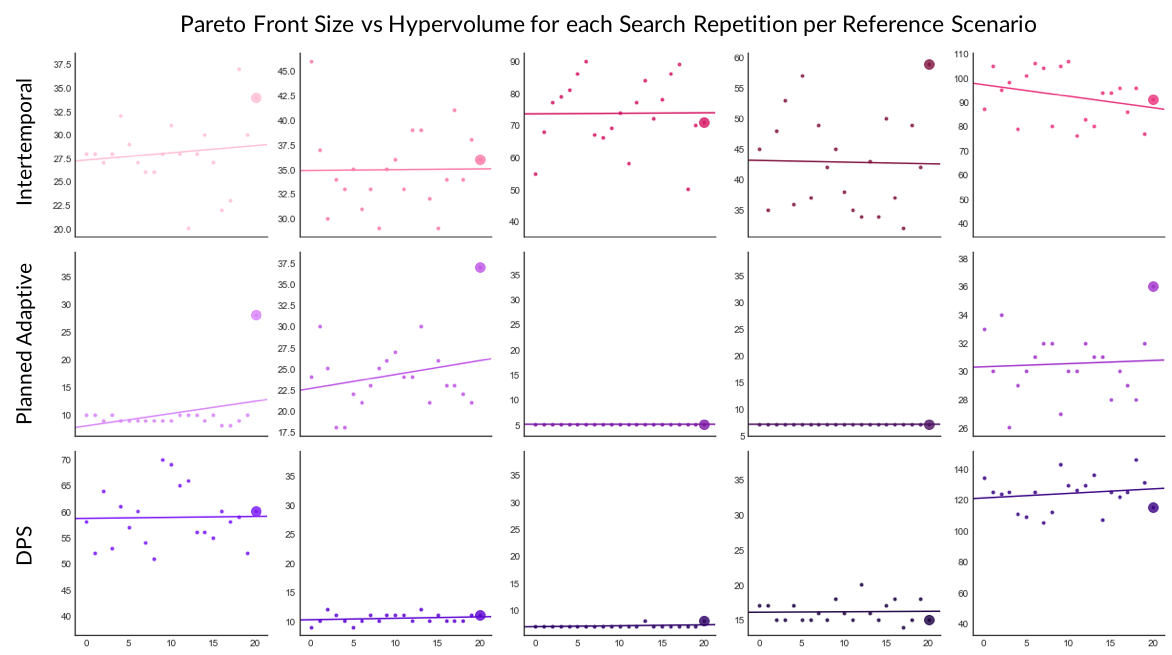
\includegraphics[width=0.95\textwidth]{appendices/seed_analysis/paretosize_multi_vs}
    \caption{The relationship between hypervolume and pareto front size across all multi-scenario MORDM analyses.}
    \label{fig:pareto-multi-versus}
\end{figure}

\begin{figure}[H]
    \centering
    
    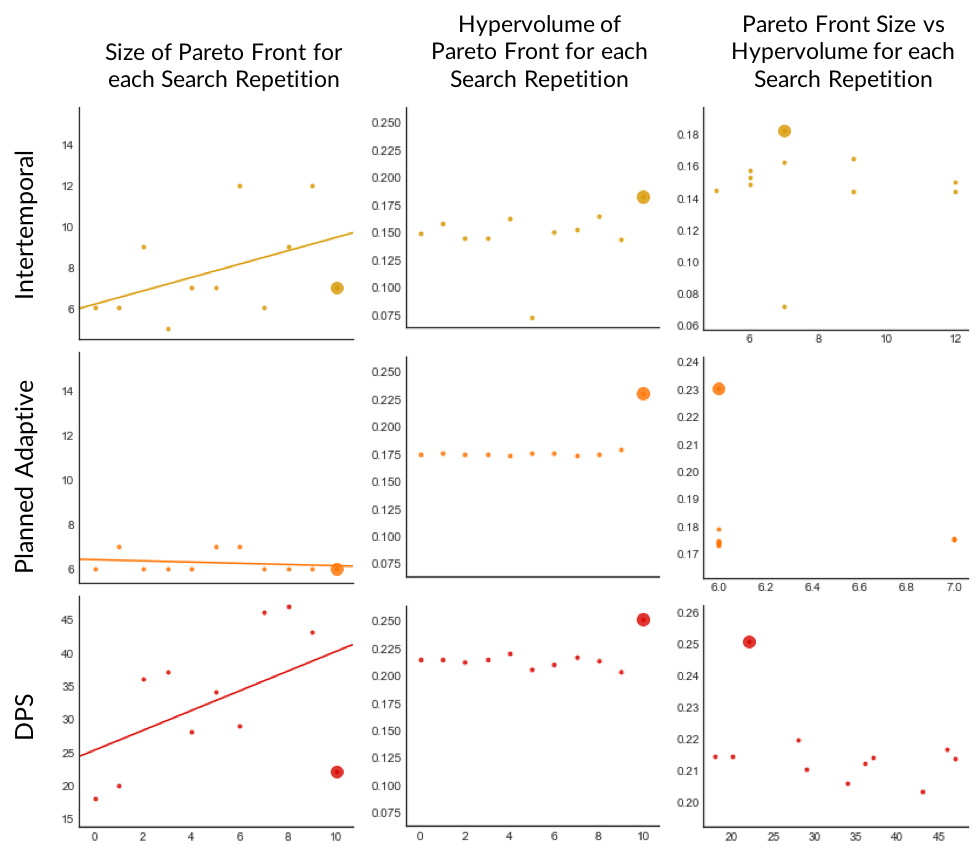
\includegraphics[width=0.75\textwidth]{appendices/seed_analysis/paretosize_moro}
    \caption[Random seed analysis for all uses of MORO]{Random seed analysis for the MORO robust decision support method. The large circle represents the set of non-dominated alternatives that combines the results from each search repetition.}
    \label{fig:pareto-moro}
\end{figure}

\section{MORO}
The results of the random seed analysis for each MORO-based analysis is shown in \cref{fig:pareto-moro} and  includes three types of plots. The first column displays the size of the identified non-dominated Pareto front size for each search repetition. The second column shows hypervolume of the final set of policy alternatives. The final column compares the size of the non-dominated set of policy alternatives to the hypervolume of each set. 

The results of the random seed analysis for each of the lake problem variations is similar to what is identified in the MORDM-based seed analysis, despite the average size of the set of non-dominated policy alternatives being considerably smaller. With respect to the intertemporal analysis, a somewhat higher diversity is achieved with a smaller set of alternatives in the combined non-dominated set. The planned adaptive DPS analysis leads to a higher diversity of policy alternatives despite maintaining a similar size in the combined set of non-dominated policy alternatives. And finally, the DPS results lead to a somewhat higher hypervolume and a combined non-dominated set size that is among the smallest obtained across all search repetitions. 
